% !TeX root = ../tfg.tex
% !TeX encoding = utf8
%
%*******************************************************
% Presupuesto
%*******************************************************

\chapter{Planificación y Presupesto}

En este capítulo se detalla como se ha organizado el trabajo, el tiempo dedicado a cada tarea y se hace un presupuesto de lo que costaría realizarlo.

\section{Planificación}
La planificación de este proyecto se ha realizado utilizando una metodología ágil, puesto que inicialmente se desconoce cuanto tiempo se va a dedicar a cada tarea. Cada semana de trabajo se proponen unos objetivos y al final se reevalúa el trabajo completado y se planifica la siguiente semana.

Inicialmente se realizó una planificación de noviembre a junio, pero fue rápidamente descartada debido a la imposibilidad de dedicarle tiempo al desarrollo de este proyecto. La planificación final se desarrolla desde mayo hasta diciembre.

\subsection{Tareas realizadas}

Aquí se resumen las principales tareas realizadas para la elaboración de la memoria:

\begin{itemize}
\item Planteamiento del problema y búsqueda de objetivos a realizar en este trabajo.
\item Búsqueda de información y lectura de libros y artículos necesarios para la elaboración y entendimiento del proyecto. 
\item Planificación del proyecto: se decidió un orden para realizar las tareas, estimando la duración de cada una y revisando esta planificación cada semana.
\item Aprendizaje sobre el funcionamiento del lenguaje de programación Julia: se dedicó un tiempo inicial al aprendizaje de la sintaxis sobre el lenguaje, conocimiento que se complementó durante el desarrollo del proyecto.
\item Implementación de los algoritmos base: Se implementaron los algoritmos base con los que luego se desarrollaría nuestra propuesta. 
\item Unión de los algoritmos basicos para crear la propuesta final.
\item Adaptación del código de DECC para utilizar agrupamiento diferencial.
\item Obtención de resultados.
\item Análisis de los resultados. 
\item Desarrollo de la memoria.
\item Revisión de la memoria
\end{itemize}

En la tabla \ref{planificacion} se puede encontrar una estimación del número de horas dedicado a cada tarea. También se puede observaren el diagrama \ref{Gaant} el orden en el que se han realizado las tareas.

\begin{table}[ht]
\centering
\caption{Planificación de tareas y horas dedicadas}
\label{planificacion}
\begin{tabular}{|l|c|}
\hline
\textbf{Tarea} & \textbf{Horas dedicadas} \\ \hline
Planteamiento del problema y objetivos & 25 \\ \hline
Búsqueda de información y lectura & 60 \\ \hline
Planificación y revisión semanal & 20 \\ \hline
Aprendizaje del lenguaje Julia & 25 \\ \hline
Implementación de algoritmos base & 100 \\ \hline
Integración de algoritmos finales & 40 \\ \hline
Adaptación del código de DECC & 25 \\ \hline
Obtención de resultados & 60 \\ \hline
Análisis de resultados & 25 \\ \hline
Elaboración de la memoria & 130 \\ \hline
Revisión de la memoria & 10 \\ \hline
\textbf{Total} & \textbf{520} \\ \hline
\end{tabular}
\end{table}

\begin{figure}[h!]
	\vspace{2cm}
    \centering
    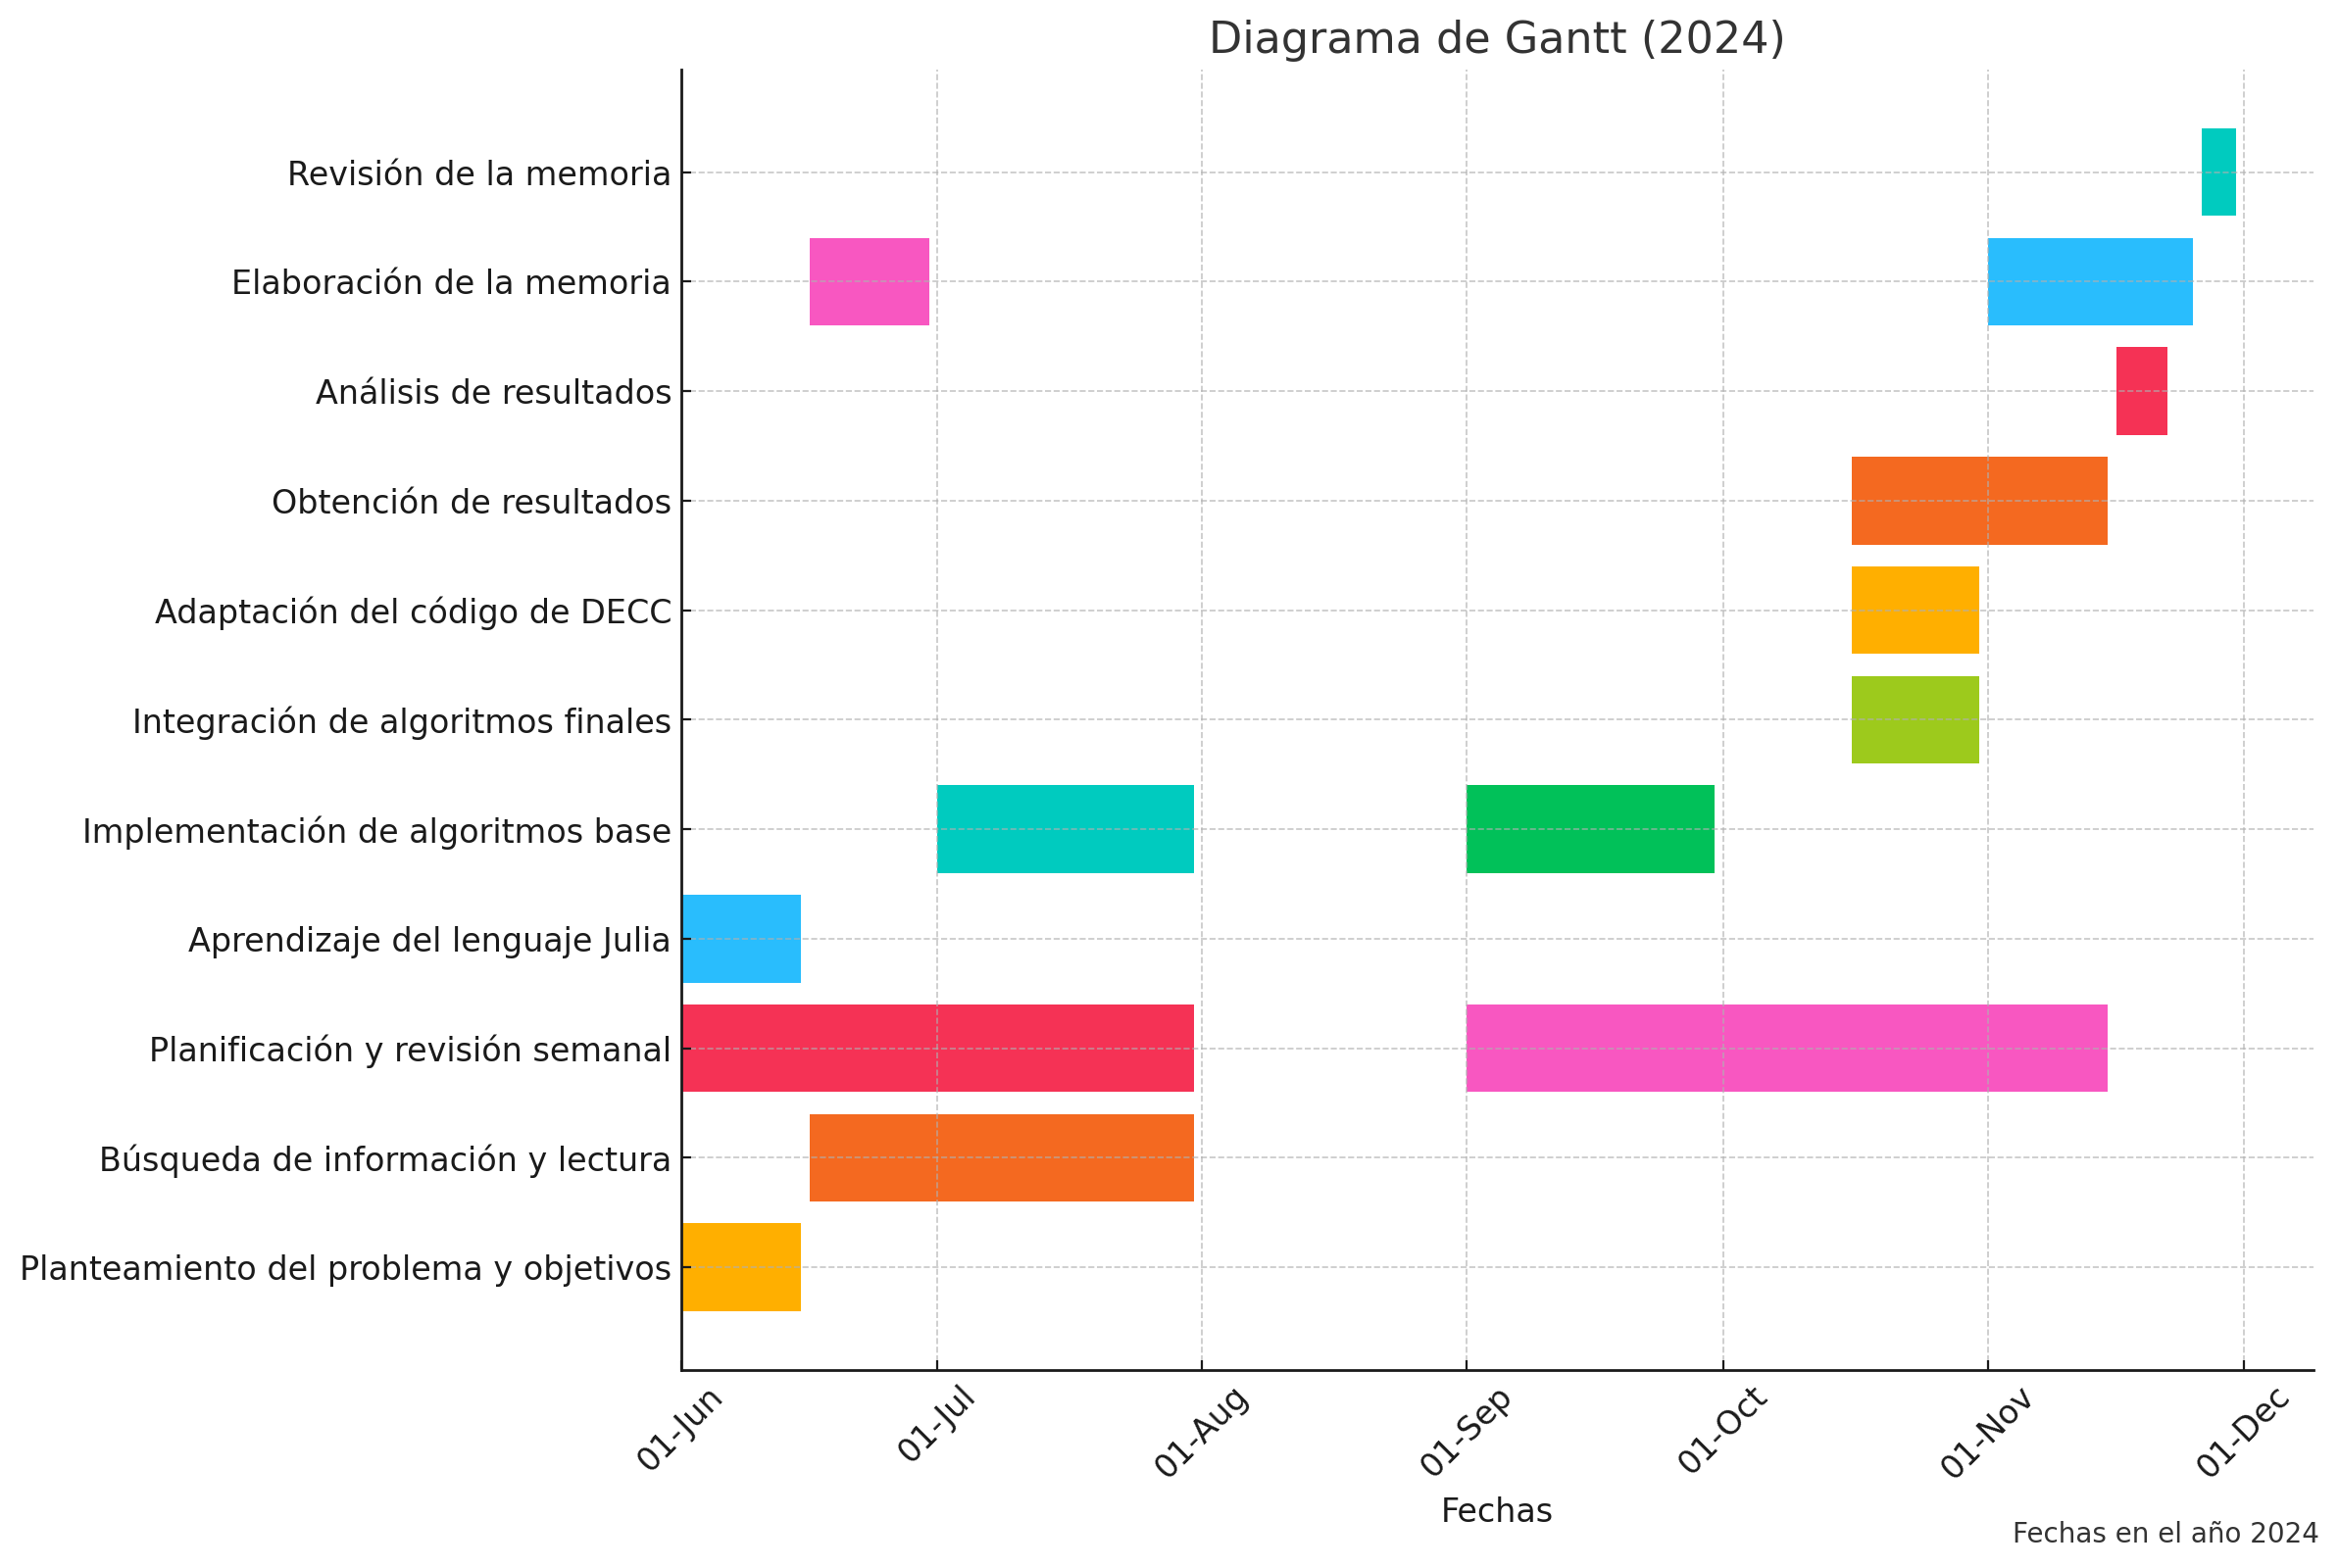
\includegraphics[width=\textwidth]{images/Diagrama_Gantt.png}
    \caption{Diagrama de Gantt de las tareas realizadas.}
    \label{Gaant}
\end{figure}

\newpage

\section{Presupuesto}

Para valorar ecónomicamente el proyecto, debemos tener en cuenta la mano de obra y el material utilizado para la elaboración del proyecto, que en este caso es solo el portátil utilizado. El precio del portátil se dividirá entre 5 años de amortización, que es la vida útil estimada del mismo multiplicado por los años de uso para la realización de este proyecto, en este caso solo uno.

El precio de la mano de obra son unos 28€ la hora.

El ordenador portátil utilizado es un ASUS ROG Zephyrus G16 (2023) GU603 con un procesador 13th Gen Intel® Core™ i9-13900H 2.6 GHz (24M  Cache, up to 5.4 GHz, 14 cores: 6 P-cores and 8 E-cores) 32 GB de RAM, con un precio de 2099€. 

Gracias a la potencia del portátil utilizado, los experimentos pudieron ejecutarse en local, lo que ahorra costes del proyecto, aunque requiere de planificar bien las horas de ejecución para no entorpecer el desarrollo del proyecto.

El cálculo del coste total del proyecto se realiza utilizando la fórmula:
\[
C_{\text{total}} = C_{\text{mano de obra}} + C_{\text{material}}
\]
donde:
\[
C_{\text{mano de obra}} = N_{\text{horas}} \times P_{\text{hora}}, \quad 
C_{\text{material}} = \frac{P_{\text{portátil}}}{A_{\text{vida útil}}} \times A_{\text{uso}}
\]

Con los datos disponibles:
- Precio de la mano de obra: \( P_{\text{hora}} = 28 \, \text{€} \)
- Horas dedicadas: \( N_{\text{horas}} = 520 \)
- Precio del portátil: \( P_{\text{portátil}} = 2099 \, \text{€} \)
- Vida útil del portátil: \( A_{\text{vida útil}} = 5 \, \text{años} \)
- Años de uso: \( A_{\text{uso}} = 1 \, \text{año} \)

El desglose de costes es el siguiente:

\begin{table}[ht]
\centering
\caption{Coste detallado del proyecto}
\label{coste_proyecto}
\begin{tabular}{|l|c|c|c|}
\hline
\textbf{Componente} & \textbf{Cantidad} & \textbf{Precio unitario (€)} & \textbf{Coste total (€)} \\ \hline
Mano de obra & 520 horas & 28 & 14.560 \\ \hline
Prorrateo del portátil & 1 año & 419.80 & 419.80 \\ \hline
\textbf{Total} & & & \textbf{14.979.80} \\ \hline
\end{tabular}
\end{table}

El presupuesto final del proyecto se fija en 14079.80€

\endinput